\documentclass[11pt,english]{article}\usepackage[]{graphicx}\usepackage[]{color}
%% maxwidth is the original width if it is less than linewidth
%% otherwise use linewidth (to make sure the graphics do not exceed the margin)
\makeatletter
\def\maxwidth{ %
  \ifdim\Gin@nat@width>\linewidth
    \linewidth
  \else
    \Gin@nat@width
  \fi
}
\makeatother

\usepackage{Sweavel}


%\VignetteIndexEntry{fdapaceVignette}
%\VignetteEngine{knitr::knitr}
\graphicspath{{figure/}}

\usepackage{palatino,avant,graphicx,color,amsmath,verbatim,url, wrapfig}
\usepackage{caption,subcaption,morefloats}
\usepackage{pdflscape}
\usepackage{amsmath, amssymb} % To use mathematics sybmols
\usepackage{verbatim}	       % To use comments
\usepackage[makeroom]{cancel} % To cross out an equation
% \usepackage{tikz}
% \usetikzlibrary{arrows,matrix,positioning}
\usepackage{listings}         % To use code listings




\usepackage [english]{babel} 
\usepackage{geometry}
\geometry{
 body={7.13in, 9.75in},
 left=1in,
 right=1in,
 top=1in,
 bottom=1in,
}

\begin{document}
% \SweaveOpts{concordance=TRUE}

\title{Functional PCA in R \\ \textit{A software primer using fdapace}}
\author{Hadjipantelis, Dai, Ji, M\"uller \& Wang - UC Davis, USA}
\maketitle
\vspace{-.61cm}

 
\lstset{
language=R,
basicstyle=\scriptsize\ttfamily,
commentstyle=\ttfamily\color{gray},
numbers=left,
numberstyle=\ttfamily\color{gray}\footnotesize,
stepnumber=1,
numbersep=6pt,
backgroundcolor=\color{white},
showspaces=false,
showstringspaces=false,
showtabs=false,
frame=false,
tabsize=2,
captionpos=b,
breaklines=true,
breakatwhitespace=true, 
escapeinside={},
keywordstyle={},
morekeywords={}
}
\section{Overview}


The basic work-flow behind the PACE approach for sparse \footnote{As a working assumption a dataset is treated as sparse if it has on average less than 20, potentially irregularly sampled, measurements per subject. A user can manually change the automatically determined \texttt{dataType} if that is necessary.} functional data is as follows (see eg. \cite{Yao05, Liu09} for more information):
\begin{enumerate}
\item Calculate the smoothed mean $\hat{\mu}$ (using local linear smoothing) aggregating all the available readings together. 
\item Calculate for each curve seperately its own raw covariance and then aggregate all these raw covariances to generate the sample raw covariance.
\item Use the off-diagonal elements of the sample raw covariance to estimate the smooth covariance.
\item Perform eigenanalysis on the smoothed covariance to obtain the estimated eigenfunctions $\hat{\phi}$ and eigenvalues $\hat{\lambda}$, then project that smoothed covariance on a positive semi-definite surface \cite{Hall2008}.
\item Use Conditional Expectation (PACE step) to estimate the corresponding scores $\hat{\xi}$. 
%ie. \newline 
%$\hat{\xi}_{ik} = \hat{E}[\hat{\xi}_{ik}|Y_i] = \hat{\lambda}_k \hat{\phi}_{ik}^T \Sigma_{Y_i}^{-1}(Y_i-\hat{\mu}_i)$.
\end{enumerate}
For densely observed functional data simplified procedures are available to obtain the eigencomponents and associated functional principal components scores (see eg. \cite{Castro86} for more information). In particular in this case we:
\begin{enumerate}
\item Calculate the cross-sectional mean $\hat{\mu}$.
\item Calculate the cross-sectional covariance surface (which is guaranteed to be positive semi-definite).
\item Perform eigenanalysis on the covariance to estimate the eigenfunctions $\hat{\phi}$ and eigenvalues $\hat{\lambda}$.
\item Use numerical integration to estimate the corresponding scores $\hat{\xi}$.
% ie. \newline
% $\hat{\xi}_{ik} =  \int_0^T [ y(t) - \hat{\mu}(t)] \phi_i(t) dt$
\end{enumerate}
% Which is part of (sparse and then dense) FPCA you believe it is the most computationally intensive?
In the case of sparse FPCA the most computational intensive part is the smoothing of the sample's raw covariance function. For this, we employ a local weighted bilinear smoother. 

A sibling MATLAB package for \texttt{fdapace} can be found in \url{http://www.stat.ucdavis.edu/PACE}.
\section{FPCA in R using fdapace}

The simplest scenario is that one has two lists \texttt{yList} and \texttt{tList} where \texttt{yList} is a list of vectors, each containing the observed values $Y_{ij}$ for the $i$th subject and \texttt{tList} is a list of vectors containing corresponding time points. In this case one uses: 

\begin{Schunk}
\begin{Sinput}
FPCAobj <- FPCA(Ly=yList, Lt=tList)
\end{Sinput}
\end{Schunk}
The generated \texttt{FPCAobj} will contain all the basic information regarding the desired FPCA.


\subsection{Generating a toy dense functional dataset from scratch}

\begin{Schunk}
\begin{Sinput}
  library(fdapace)
  #devtools::load_all('.') # So we use the new interfaces

  # Set the number of subjects (N) and the
  # number of measurements per subjects (M) 
  N <- 200;   
  M <- 100;
  set.seed(123)

  # Define the continuum
  s <- seq(0,10,length.out = M)
 
  # Define the mean and 2 eigencomponents
  meanFunct <- function(s) s + 10*exp(-(s-5)^2)
  eigFunct1 <- function(s) +cos(2*s*pi/10) / sqrt(5)
  eigFunct2 <- function(s) -sin(2*s*pi/10) / sqrt(5)
  
  # Create FPC scores
  Ksi <- matrix(rnorm(N*2), ncol=2);
  Ksi <- apply(Ksi, 2, scale)
  Ksi <- Ksi %*% diag(c(5,2))
 
  # Create Y_true
  yTrue <- Ksi %*% t(matrix(c(eigFunct1(s),eigFunct2(s)), ncol=2)) + t(matrix(rep(meanFunct(s),N), nrow=M))
\end{Sinput}
\end{Schunk}

\subsection{Running FPCA on a dense dataset }
\begin{minipage}[l]{0.5\textwidth}
\begin{Schunk}
\begin{Sinput}
  L3 <- MakeFPCAInputs(IDs = rep(1:N, each=M),tVec=rep(s,N), t(yTrue))
  FPCAdense <- FPCA(L3$Ly, L3$Lt)   
  
  # Make a basic diagnostics plot
  plot(FPCAdense)
\end{Sinput}
\begin{Sinput}
  # Find the standard deviation associated with each component
  sqrt(FPCAdense$lambda)
\end{Sinput}
\begin{Soutput}
[1] 5.050606 1.999073
\end{Soutput}
\end{Schunk}
\end{minipage}
\begin{minipage}[r]{0.495\textwidth}
  \includegraphics[width=\textwidth]{denseSim-1.pdf}
\end{minipage}

\subsection{Running FPCA on a sparse and noisy dataset }

\begin{minipage}[l]{0.51\textwidth}
\begin{Schunk}
\begin{Sinput}
  # Create sparse sample  
  # Each subject has one to five readings (median: 3)
  set.seed(123)
  ySparse <- Sparsify(yTrue, s, sparsity = c(1:5))
    
  # Give your sample a bit of noise 
  ySparse$yNoisy <- lapply(ySparse$Ly, function(x) x + 0.5*rnorm(length(x))) 
  
  
  # Do FPCA on this sparse sample
  # Notice that sparse FPCA will smooth the data internally (Yao et al., 2005)
  # Smoothing is the main computational cost behind sparse FPCA
  FPCAsparse <- FPCA(ySparse$yNoisy, ySparse$Lt, list(diagnosticsPlot = TRUE))  
\end{Sinput}
\end{Schunk}
\end{minipage}
\begin{minipage}[r]{0.49\textwidth}
  \includegraphics[width=\textwidth]{sparseSim-1.pdf}
\end{minipage}

\newpage
\section{Further functionality}

%\begin{itemize}

\texttt{FPCA} calculates the bandwidth utilized by each smoother using generalised cross-validation or $k$-fold cross-validation automatically. Dense data are not smoothed by default. The argument \texttt{methodMuCovEst} can be switched between \texttt{smooth} and \texttt{cross-sectional} if one wants to utilize different estimation techniques when work with dense data. 
%Which was the bandwidth used to calculate the smoothed mean in \texttt{FPCAdense} and in \texttt{FPCAsparse}? 
%Was the bandwidth used for the calculation of $\hat{\mu}$ larger or smaller than the bandwidth used for smoothing the covariance surface? (Check \texttt{...\$bwMu} and \texttt{...\$bwCov} respectively).\newline
The bandwidth used for estimating the smoothed mean and the smoothed covariance are available under \texttt{...\$bwMu} and \texttt{...\$bwCov} respectively. Users can nevertheless provide their own bandwidth estimates:
\begin{Schunk}
\begin{Sinput}
 FPCAsparseMuBW5 <- FPCA(ySparse$yNoisy, ySparse$Lt, optns= list(userBwMu = 5)) 
\end{Sinput}
\end{Schunk}
Visualising the fitted trajectories is a good way to see if the new bandwidth made any sense:
%par(mfrow=c(1,2))
\begin{Schunk}
\begin{Sinput}
CreatePathPlot( FPCAsparse, subset = 1:3, main = "GCV bandwidth", pch = 16)
CreatePathPlot( FPCAsparseMuBW5, subset = 1:3, main = "User-defined bandwidth", pch = 16)
\end{Sinput}


{\centering \includegraphics[width=.45\linewidth]{figure/bwChoice-1} \includegraphics[width=.45\linewidth]{figure/bwChoice-2} 

}

\end{Schunk}
%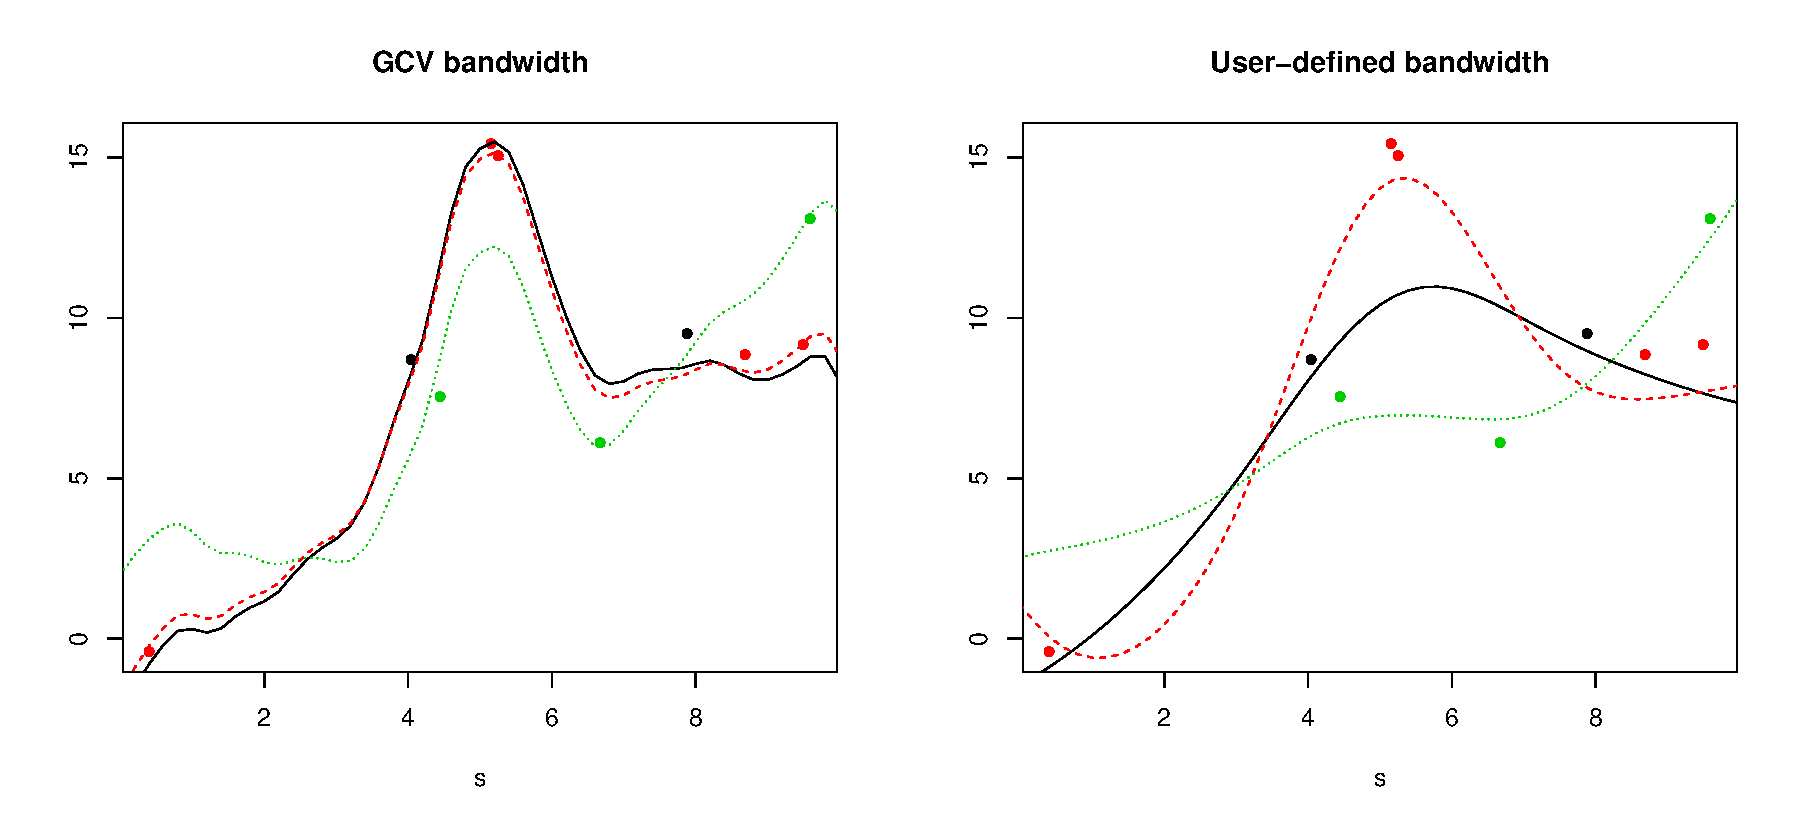
\includegraphics[width=\textwidth]{DifferentBandwidths}
\texttt{FPCA} uses a Gaussian kernel when smoothing sparse functional data; other kernel types (eg. Epanechnikov/\texttt{epan}) are also available (see \texttt{?FPCA}). The kernel used for smoothing the mean and covariance surface is the same. It can be found under \texttt{...\$optns\$kernel} of the returned object. For instance, one can switch the default Gaussian kernel (\texttt{gauss}) for a rectangular kernel (\texttt{rect}) as follows:

\begin{Schunk}
\begin{Sinput}
 FPCAsparseRect <- FPCA(ySparse$yNoisy, ySparse$Lt, optns = list(kernel = 'rect')) # Use rectangular kernel
\end{Sinput}
\end{Schunk}

\texttt{FPCA} returns automatically the smallest number of components required to explain 99.99\% of a sample's variance. Using the function \texttt{selectK} one can determine the number of relevant components according to AIC, BIC or a different Fraction-of-Variance-Explained threshold. For example:
\begin{Schunk}
\begin{Sinput}
SelectK( FPCAsparse, criterion = 'FVE', FVEthreshold = 0.95) # k = 2
SelectK( FPCAsparse, criterion = 'AIC') # k = 2
\end{Sinput}
\end{Schunk}
When working with functional data (usually not very sparse) the estimation of derivatives is often of interest. Using \texttt{fitted.FPCA} one can directly obtain numerical derivatives by defining the appropriate order \texttt{p}; \texttt{fdapace} provides for the first two derivatives (\texttt{p = 1} or \texttt{2}). Because the numerically differentiated data are smoothed the user can define smoothing specific arguments (see \texttt{?fitted.FPCA} for more information); the derivation is done by using the derivative of the linear fit. Similarly using the function  \texttt{FPCAder}, one can augment an \texttt{FPCA} object with functional derivatives of a sample's mean function and eigenfunctions. 

\begin{Schunk}
\begin{Sinput}
fittedCurvesP0 <- fitted(FPCAsparse) # equivalent: fitted(FPCAsparse, derOptns=list(p = 0));
# Get first order derivatives of fitted curves, smooth using Epanechnikov kernel
fittedCurcesP1 <- fitted(FPCAsparse, derOptns=list(p = 1, kernelType = 'epan')) 
\end{Sinput}
\end{Schunk}

\section{A real-world example}

We use the \texttt{medfly25} dataset that this available with \texttt{fdapace} to showcase \texttt{FPCA} and its related functionality. \texttt{medfly25} is a dataset containing the eggs laid from 789 medflies (Mediterranean fruit flies, Ceratitis capitata) during the first 25 days of their lives. It is a subset of the dataset used by Carey at al. (1998) \cite{Carey98}; only flies having lived at least 25 days are shown. The data are rather noisy, dense and with a characteristic flat start. For that reason in contrast with above we will use a smoothing estimating procedure despite having dense data.   

\begin{minipage}[l]{0.5\textwidth}
\begin{Schunk}
\begin{Sinput}
  # load data
  data(medfly25)

  # Turn the original data into a list of paired amplitude and timing lists
  Flies <- MakeFPCAInputs(medfly25$ID, medfly25$Days, medfly25$nEggs) 
  fpcaObjFlies <- FPCA(Flies$Ly, Flies$Lt, list(diagnosticsPlot = TRUE, methodMuCovEst = 'smooth', userBwCov = 2)) 
\end{Sinput}
\end{Schunk}
\end{minipage}
\begin{minipage}[r]{0.495\textwidth}
  \includegraphics[width=\textwidth]{medfly-1.pdf}
\end{minipage} 

Based on the scree-plot we see that the first three components appear to encapsulate most of the relevant variation. The number of eigencomponents to reach a $99.99\%$ FVE is $11$ but just $3$ eigencomponents are enough to reach a $95.0\%$. We can easily inspect the following visually, using the \texttt{CreatePathPlot} command.
 % par(mfrow=c(1,2))
\begin{Schunk}
\begin{Sinput}
  CreatePathPlot(fpcaObjFlies, subset = c(3,5,135), main = 'k = 11', pch = 4); grid()
  CreatePathPlot(fpcaObjFlies, subset = c(3,5,135), k = 3, main = 'k = 3', pch = 4) ; grid()  
\end{Sinput}


{\centering \includegraphics[width=.45\linewidth]{figure/k-1} \includegraphics[width=.45\linewidth]{figure/k-2} 

}

\end{Schunk}

%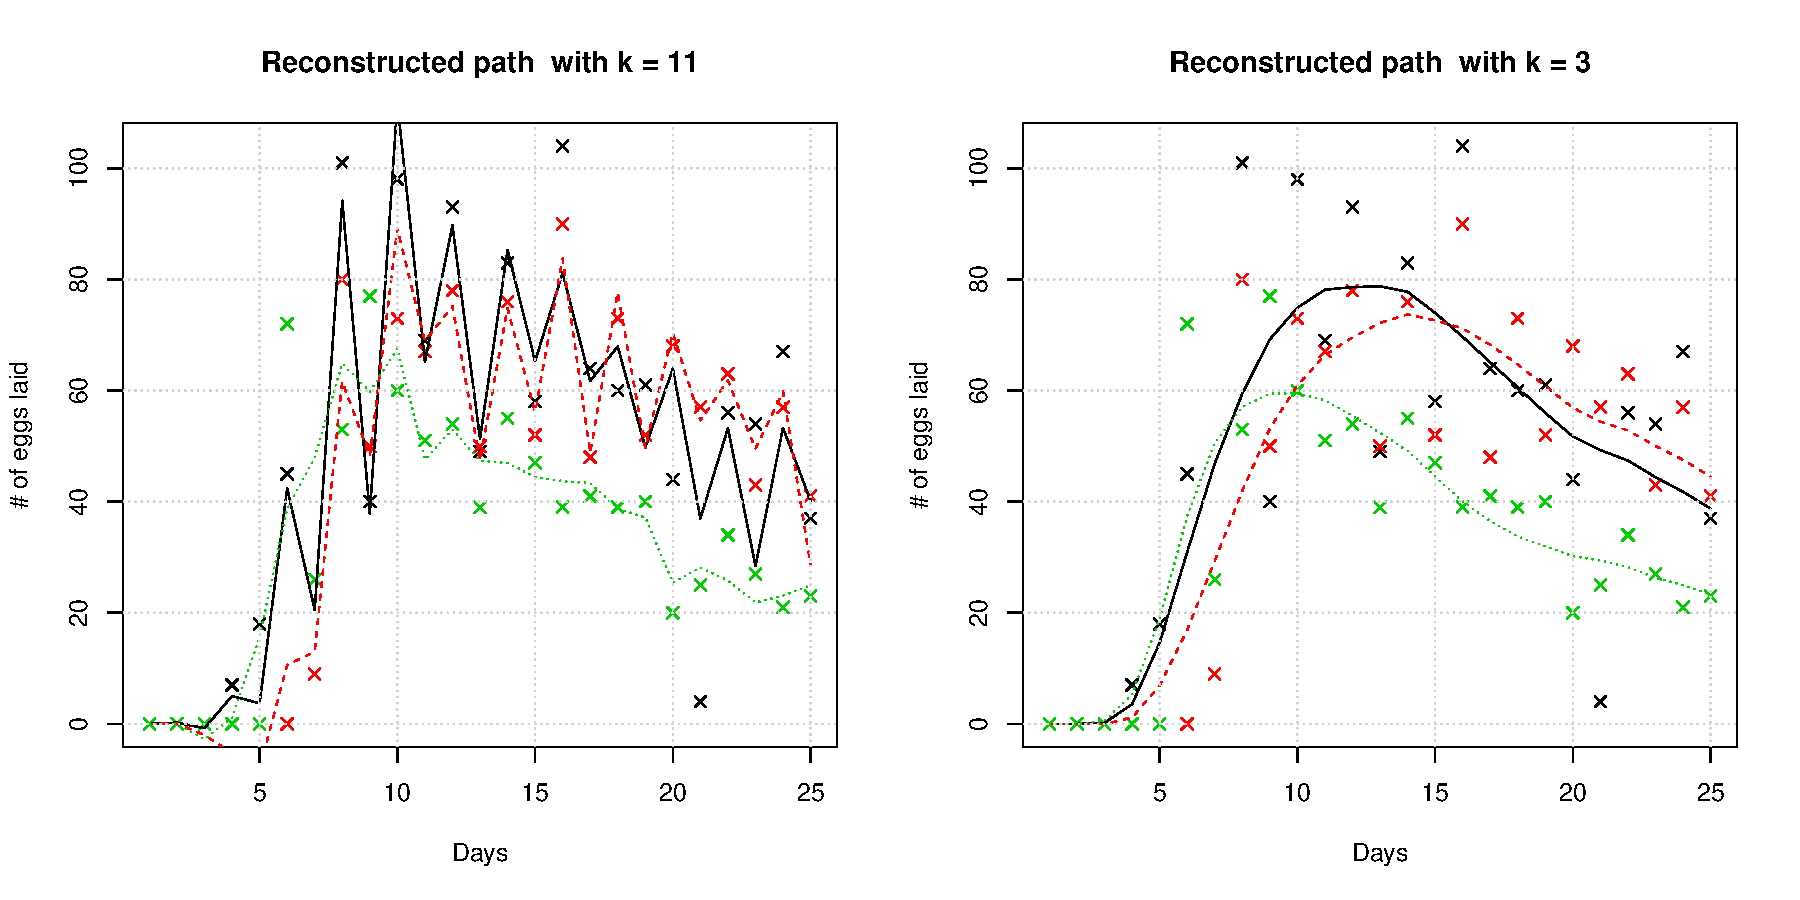
\includegraphics[width=0.9\textwidth]{PathFlies}

One can perform outlier detection \cite{Febrero2007} as well as visualize data using a functional box-plot. To achieve these tasks one can use the functions \texttt{CreateOutliersPlot} and \texttt{CreateFuncBoxPlot}. Different ranking methodologies (KDE, bagplot \cite{Rousseeuw1999,Hyndman2010} or point-wise) are available and can potentially identify different aspects of a sample. For example here it is notable that the  kernel density estimator \texttt{KDE} variant identifies two main clusters within the main body of sample. By construction the \texttt{bagplot} method would use a single \textit{bag} and this feature would be lost. Both functions return a (temporarily) invisible copy of a list containing the labels associated with each of sample curve. \texttt{CreateOutliersPlot} returns a (temporarily) invisible copy of a list containing the labels associated with each of sample curve.
%  par(mfrow=c(1,2))
\begin{Schunk}
\begin{Sinput}
  CreateOutliersPlot(fpcaObjFlies, optns = list(k = 3, variant = 'KDE'))
  CreateFuncBoxPlot(fpcaObjFlies, xlab = 'Days', ylab = '# of eggs laid', optns = list(k =3, variant='bagplot'))
\end{Sinput}


{\centering \includegraphics[width=.4\linewidth]{figure/outlier-1} \includegraphics[width=.4\linewidth]{figure/outlier-2} 

}

\end{Schunk}

Functional data lend themselves naturally to questions about their rate of change; their derivatives. As mentioned previously using \texttt{fdapace} one can generate estimates of the sample's derivatives (\texttt{fitted.FPCA}) or the derivatives of the principal modes of variation (\texttt{FPCAder}). In all cases, one defines a \texttt{derOptns} list of options to control the derivation parameters. Getting derivatives is obtained by using a local linear smoother as above. 

\begin{Schunk}
\begin{Sinput}
  CreatePathPlot(fpcaObjFlies, subset = c(3,5,135), k = 3, main = 'k = 3', showObs = FALSE) ; grid() 
  CreatePathPlot(fpcaObjFlies, subset = c(3,5,135), k = 3, main = 'k = 3', showObs = FALSE, derOptns = list(p = 1, bw = 1.01 , kernelType = 'epan') ) ; grid() 
\end{Sinput}


{\centering \includegraphics[width=.45\linewidth]{figure/deriv-1} \includegraphics[width=.45\linewidth]{figure/deriv-2} 

}

\end{Schunk}

We note that if finite support kernel types are used (eg. \texttt{rect} or \texttt{epan}), bandwidths smaller than the distance between two adjacent points over which the data are registered onto will lead to (expected) \texttt{NaN} estimates. In case of dense data, the grid used is (by default) equal to the grid the data were originally registered on; in the case of sparse data, the grid used (by default) spans the range of the sample's supports and uses 51 points. A user can change the number of points using the argument \texttt{nRegGrid}.  
One can investigate the effect a particular kernel type (\texttt{kernelType}) or bandwidth size (\texttt{bw}) has on the generated derivatives by using the function \texttt{CreateDiagnosticsPlot} but this time providing a relevant \texttt{derOptns} list. This will generate estimates about the mean function $\mu(t)$ as well as the first two principal modes of variation $\phi_1(t)$ and $\phi_2(t)$ for different multiples of \texttt{bw}. 

\begin{Schunk}
\begin{Sinput}
fpcaObjFlies79 <- FPCA(Flies$Ly, Flies$Lt, list(nRegGrid = 79, methodMuCovEst = 'smooth', userBwCov = 2)) # Use 79 equidistant points for the support
CreateBWPlot(fpcaObjFlies79 , derOptns = list(p = 1, bw = 2.0 , kernelType = 'rect') )
\end{Sinput}


{\centering \includegraphics[width=\maxwidth]{figure/bwPlot-1} 

}

\end{Schunk}

%' \begin{minipage}[l]{0.5\textwidth}
%' <<eval=FALSE>>= 
%' fpcaObjFlies79 <- FPCA(Flies$Ly, Flies$Lt, list(diagnosticsPlot = TRUE, nRegGrid = 79, methodMuCovEst = 'smooth', userBwCov = 2)) # Use 79 equidistant points for the support
%' 
%' CreateBWPlot(fpcaObjFlies79 , derOptns = list(p = 1, bw = 2.0 , kernelType = 'rect') )
%' @
%' \end{minipage}
%' \begin{minipage}[r]{0.495\textwidth}
%'   \includegraphics[width=\textwidth]{bwPlot-1.pdf}
%' \end{minipage}
%' \includegraphics[width=0.9\textwidth]{bwPlot-2.pdf}



As the \texttt{medfly} sample is dense we can immediately use standard multivaritte clustering functionality to identify potential subgroups within it; the function  \texttt{FClust} is the wrapper around the clustering functionality provided by \texttt{fdapace}.  By default \texttt{FClust} utilises a Gaussian Mixture Model approach based on the package \texttt{Rmixmod} \cite{Biernacki2006}, as a general rule clustering optimality is based on negative entropy criterion. In the \texttt{medfly} dataset clustering the data allows to immediately recognise a particular subgroup of flies that lay no or very few eggs during the period examined.
 
\begin{Schunk}
\begin{Sinput}
A <- FClust(Flies$Ly, Flies$Lt, optnsFPCA = list(methodMuCovEst = 'smooth', userBwCov = 2, FVEthreshold = 0.90))
\end{Sinput}
\begin{Soutput}
Error in eval(expr, envir, enclos): could not find function "FClust"
\end{Soutput}
\begin{Sinput}
B <- FClust(Flies$Ly, Flies$Lt, optnsFPCA = list(methodMuCovEst = 'smooth', userBwCov = 2, FVEthreshold = 0.90), k = 2)
\end{Sinput}
\begin{Soutput}
Error in eval(expr, envir, enclos): could not find function "FClust"
\end{Soutput}
\begin{Sinput}
#  A$clusterObj@bestResult@criterionValue is greater than B$clusterObj@bestResult@criterionValue
CreatePathPlot( fpcaObjFlies, k=2, showObs=FALSE, lty=1, col= B$cluster, xlab = 'Days', ylab = '# of eggs laid')
\end{Sinput}
\begin{Soutput}
Error in CreatePathPlot(fpcaObjFlies, k = 2, showObs = FALSE, lty = 1, : object 'B' not found
\end{Soutput}
\begin{Sinput}
grid()
\end{Sinput}
\begin{Soutput}
Error in int_abline(a = a, b = b, h = h, v = v, untf = untf, ...): plot.new has not been called yet
\end{Soutput}
\end{Schunk}

\bibliographystyle{plain}
\bibliography{roxygen}%


\end{document}
